\section{Sparsity}
\label{sec:ch7:sparse}

In Section \ref{sec:ch4:prop-net:density}, you learned about a very important descriptive property of networks called the network density. An understanding of the network density gives us the ability to describe another extremely ubiquitous property of networks: the network sparsity. 


To understand this section, we're going to use the working example in Remark \ref{box:ch7:sparse}:

\begin{floatingbox}[h]\caption{Sparse network example}
\label{box:ch7:sparse}
The nodes of the network will represent academic scholars in computer science from $K$ universities. For every university, there are $100$ scholars investigated for an arbitrary sample of researchers in the community. An edge exists if a pair of researchers have co-authored a paper together. Therefore, researchers who work with more people will have more edges, and consequently, a higher node degree.

Most researchers publish a lot of papers with their working groups; the within-university probability will be $1$, but the between-university probability will be $0.01$ (the network is extremely homophilic).

$95\%$ of the researchers will prot\'eg\'es; they are not yet running a lab, so most of their work occurs with close collaborators at their university. These researchers have a degree-correction factor that is $Beta(1, 4)$ distributed; this just means that their degree-correction factors will be between $0$ and $1$, but will tend to be quite low (on average, $\frac{1}{1 + 4} = \frac{1}{5}$). 

On the other hand, $5\%$ of the researchers will be lab leaders; they tend to spend a lot of time working with researchers both within and outside of their university. These researchers will have a degree-correction factors that is $Beta(2, 1)$ distributed; again this means the degree-correction factors will be between $0$ and $1$, but will tend to be quite high (on average, $\frac{2}{1 + 2} = \frac{2}{3}$).
\end{floatingbox}


We can produce our network like this, which is very similar to how we generated a $DCSBM_n(\vec z, \vec \theta, B)$ sample in Section \ref{sec:ch5:dcsbm}. We separate out the construction of the probability matrix here so that we don't have to sample the entire network every time, which gets very cumbersome:

\begin{lstlisting}[style=python]
import numpy as np
from graspologic.simulations import sample_edges
from graphbook_code import generate_sbm_pmtx
    
def academic_pmtx(K):
    """
    Produce probability matrix for academic example.
    """
    nk = 100
    n = K*nk
    # get the community assignments
    zs = [k for k in range(1, K + 1) for i in range(nk)]
    # randomly generate proteges and lab leaders
    unif_choices = np.random.uniform(size=n)
    thetas = np.zeros((n,))
    # 90% are proteges
    thetas[unif_choices > .1] = np.random.beta(1, 5, size=(unif_choices > .1).sum())
    # 10% are lab leaders
    thetas[unif_choices <= .1] = np.random.beta(2, 1, size=(unif_choices <= .1).sum())
    # define block matrix
    B = 0.01*np.ones((K, K))
    np.fill_diagonal(B, 1)
    # generate probability matrix for SBM
    Pp = generate_sbm_pmtx(zs, B)
    thetas = thetas.reshape(-1)
    Theta = np.diag(thetas)
    # adjust probability matrix for SBM by degree-corrections
    P = Theta @ Pp @ Theta.transpose()
    return P

def academic_example(K):
    P = academic_pmtx(K)
    return sample_edges(P)
\end{lstlisting}

First, we will introduce a few concepts about sparsity, and then we’ll tie in how this comes into play with learning from your network data. As a quick forenote, this section is going to assume that you have a working knowledge of the concept of a sequence, and that you have conceptualized algorithmic complexity and asymptotic notation at some point in your work life. If you need a quick refresher on asymptotic notation, we'd recommend that you give the wikipedia page a read-over \cite{bigonotation}. We summarized the big concepts that we will touch on in Remark \ref{box:ch7:asy}. Finally, we will see how the typical modes that network data are stored and analyzed can benefit if we know ahead of time that the network is sparse.


\begin{floatingbox}[h]\caption{Asymptotic notation}
\label{box:ch7:asy}
Asymptotic notation is a description of what happens at the limits of the domains of functions. Suppose that $f(x)$ and $g(x)$ are two functions, that are defined for real values $x$. Common asymptotic notations include:
\begin{enumerate}
    \item $f(x) = \mathcal O(g(x))$: ``$f(x)$ is big-O of $g(x)$'' means that $g(x)$ is a rate that upper-bounds $f(x)$. Formally, there exists a constant multiplier $M$ and a value $x_M$ where for any value $x \geq x_M$:
    \begin{align*}
        |f(x)| \leq Mg(x).
    \end{align*}
    The idea here is that $g(x)$ is an upper bound for $f(x)$ (for some arbitrary constant $M$).
    \item $f(x) = \smallO(g(x))$: ``$f(x)$ is little-o of $g(x)$'' means that for \textit{any} positive constant $\epsilon$, there exists an $x_\epsilon$ where for any value $x \geq x_\epsilon$:
    \begin{align*}
        |f(x)| \leq \epsilon g(x).
    \end{align*}
    The intuition here is that $g(x)$ is growing so much faster than $f(x)$ for large values of $x$, that if we chose any arbitrarily miniscule multiplier $\epsilon$, we could find a value $x_\epsilon$ where $g(x)$ is still going to be much larger than $|f(x)|$, even after we rescale by $\epsilon$, for any $x \geq x_{\epsilon}$.
\end{enumerate}
The key distinction between big-$\mathcal O$ and little-$\smallO$ notation is that for big-$\mathcal O$ notation, we only need to be able to find a single choice of a constant $M$ where the inequality holds. However, for little-$\smallO$ notation, the relationship can be found for any choice of a constant $\epsilon$. 

In this sense, for a function $f(x)$ to be big-$\mathcal O$ of $g(x)$, it can be growing at the same speed, or slower, than $g(x)$, just as long as it is eventually (for all $x \geq x_M$) multiplicatively close for some factor $M$. On the other hand, for $f(x)$ to be little-$\smallO$ of $g(x)$, it must be so much smaller than $g(x)$ that we could always go ``farther out'' in the domain and have the inequality hold.
\end{floatingbox}

\subsection{Formal definitions of sparse networks}

Let's imagine that we have a collection of random networks $\left\{\mathbf A^{(1)}, \mathbf A^{(2)}, \hdots \right\}$. This collection is called a \textit{sequence of random networks}, because we assume that the collection contains a random networks $\mathbf A^{(n)}$ for every possible indexing value of $n$ (extending all the way out to infinity). In this case, the random network $\mathbf A^{(n)}$ is going to be a network with $n$ nodes. It is called a \textit{sequence} because there is an order to the collection (the number of nodes in the network).

\paragraph*{A formal definition of sparsity}
A sequence of networks is \textit{sparse} if:
\begin{align*}
    \mathbb E\left[\sum_{j > i}\mathbf a_{ij}^{(n)}\right] = \smallO\left(\binom n 2\right).\numberthis \label{eqn:ch7:density:def1}
\end{align*}
For a network $\mathbf A^{(n)}$ with $n$ nodes, $\mathbb E\left[\sum_{j > i}\mathbf a_{ij}^{(n)}\right]$ can be thought of as the expected number of edges in the network, and $\binom n 2$ is the (constant) number of potential edges in the network. With the characterization of asymptotic notation in Remark \ref{box:ch7:asy} in mind, what this means is that, ``the expected number of edges in the networks grows much slower than the number of potential edges''.

Note that by the definition of asymptotic notation $\smallO(\cdot)$, what this means is that for any value $\epsilon > 0$, we can find an $n_\epsilon$ where for all $n \geq n_\epsilon$:
\begin{align*}
    \mathbb E\left[\sum_{j > i}\mathbf a_{ij}^{(n)}\right] &\leq \epsilon \binom{n}{2}. \numberthis\label{eqn:ch7:density:def1_condition}
\end{align*}

Let's see how this looks for our random networks described in Remark \ref{box:ch7:sparse}. Note that the probability matrix has some element of randomness to it (the degree-correction factors), so you won't get exactly the same results every time, but it should give you a good idea of what to expect. We'll run the simulation and average over $30$ repetitions per setting to account for this added source of randomness:
\begin{lstlisting}[style=python]
import pandas as pd

results = []
nrep = 30
for K in np.linspace(2, 64, 10).astype(int):
    for j in range(nrep):
        P = academic_pmtx(K)
        n = P.shape[0]
        results.append({"Count": np.triu(P).sum(), "Edges": "Expected", 
                        "#Nodes": n, "Index": j})
        results.append({"Count": n*(n - 1)/200, "Edges": "Potential/100",
                        "#Nodes": n, "Index": j})

df = pd.DataFrame(results)
df_mean=df.groupby(["Edges", "#Nodes"])[["Count"]].mean()
\end{lstlisting}

Note that in the above code, we normalized the number of potential edges by a factor of $100$ so that these two values could exist on the same plot (the number of potential edges grows really quickly). We can plot the number of potential edges $\binom n 2$ against the number of expected edges like this:
\begin{lstlisting}[style=python]
sns.lineplot(data=df, x="#Nodes", y="Count", hue="Edges")
\end{lstlisting}
The result is shown in Figure \ref{fig:ch7:density:sparsity}(A). Note that the number of potential edges is growing exponentially (dashed line), but the number of expected edges (solid line) looks like it is only growing linearly with the number of nodes. For instance, if we were to choose a value $\epsilon = 0.0064$, we could look at the plot, and go to around $n_\epsilon = 1000$ nodes where the number of potential edges is around $500000$ and the number of expected edges is around $n_\epsilon = 3200$ (the vertical, faint gray line). If we take any $n \geq n_{\epsilon}$, it will be the case that the number of expected edges is less than $\epsilon\cdot$ the number of potential edges. We could repeat this process for any choice of $\epsilon$, however small (noting that we might have to make our simulation a lot higher number of nodes for really small values of $\epsilon$).

\begin{figure}
    \centering
    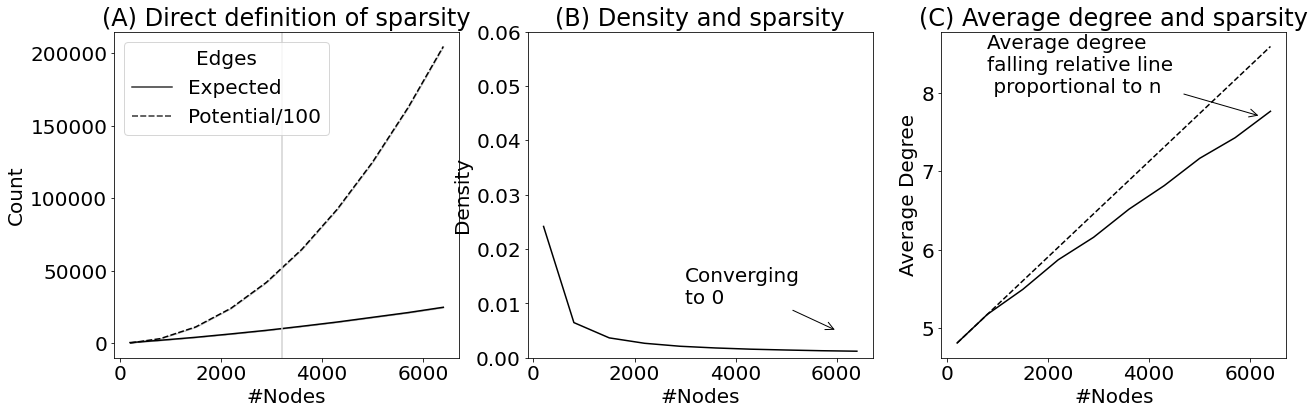
\includegraphics[width=\linewidth]{applications/ch7/Images/sparse_nets.png}
    \caption[Conceptualizing sparse networks]{\textbf{(A)} the direct definition of sparsity, \textbf{(B)} the equivalent definition of sparsity using the expected network density, \textbf{(C)} the equivalent definition of sparsity using the expected average node degree. Network sparsity has very specific definitions detailed in this section that must be proven out mathematically; illustrative plots like these are helpful to develop intuition for network sparsity, but are insufficient to prove that a sequence of random networks is sparse.}
    \label{fig:ch7:density:sparsity}
\end{figure}

\paragraph*{Relating sparsity to the network density}

Let's assume that we are given a value $\epsilon > 0$, and the $n_\epsilon$ such that the Equation \eqref{eqn:ch7:density:def1_condition} holds for all $n \geq n_\epsilon$.

Dividing through by $\binom n 2$ we see that for this $\epsilon$ and $n_\epsilon$ pair, that it is also the case that for all $n \geq n_\epsilon$:
\begin{align*}
    \mathbb E\left[density\left(\mathbf A^{(n)}\right)\right] &= \frac{\mathbb E\left[\sum_{j > i}\mathbf a_{ij}^{(n)}\right]}{\binom n 2} \leq \epsilon,\numberthis\label{eqn:ch7:sparse:density}
\end{align*}
where we simply used the definition of the expected density from Section \ref{sec:ch5:prop:rndens}. This shows that another equivalent characterization of sparse networks is that:
\begin{align*}
    \mathbb E\left[density\left(\mathbf A^{(n)}\right)\right] &= \smallO(1).
\end{align*}
or that, ``the expected density is decreasing to $0$ as the number of nodes grows''. 

We can repeat this with our experimental data by simply dividing the number of expected edges by the number of potential edges (adjusting for the normalization we made), like so:
\begin{lstlisting}[style=python]
df_wide = pd.pivot(df_mean.reset_index(), index="#Nodes", columns="Edges", values="Count")
df_wide["Density"] = df_wide["Expected"]/(100*df_wide["Potential/100"])
df_wide = df_wide.reset_index()
# plot it
sns.lineplot(data=df_wide, x="#Nodes", y="Density", color="black")
\end{lstlisting}

In the plot in Figure \ref{fig:ch7:density:sparsity}(B), we can see that for any choice of $\epsilon$, it looks like we could choose some value $n_\epsilon$ where the expected density is less than $\epsilon$.

\paragraph*{Relating sparsity to the expected average node degree}

Remember in Section \ref{sec:ch5:prop:rndens}, that we wrote the expected network density as:
\begin{align*}
    \mathbb E\left[density\left(\mathbf A^{(n)}\right)\right] &= \frac{\mathbb E[\mathbf d^{(n)}]}{n - 1},
\end{align*}
where $\mathbb E[\mathbf d^{(n)}] = \frac{1}{n}\sum_{i = 1}^n \mathbb E[\mathbf d_i^{(n)}]$ was the expected average node degree. 

Similarly, we can write that for the same choice of $\epsilon$ and $n_\epsilon$ as in Equation \eqref{eqn:ch7:sparse:density}, that if Equation \eqref{eqn:ch7:sparse:density} holds for any $\epsilon > 0$ and $n \geq n_\epsilon$, that it is also the case that:
\begin{align*}
    \mathbb E\left[density\left(\mathbf A^{(n)}\right)\right] = \frac{\mathbb E[\mathbf d^{(n)}]}{n - 1} &\leq \epsilon \\
    \Rightarrow \mathbb E[\mathbf d^{(n)}] &\leq (n - 1)\epsilon \leq n\epsilon,
\end{align*}
where the last inequality is because $\epsilon > 0$, so $(n - 1)\epsilon \leq n\epsilon$. This shows that in a sparse collection of networks, the expected node degree $\mathbb E\left[\mathbf d^{(n)}\right] = \smallO(n)$. 

This gives us our final equivalent characterization of sparse networks as networks where ``the expected average degree grows sublinearly with the number of nodes in the network''.

In the plot in Figure \ref{fig:ch7:density:sparsity}(C), we can see a diagonal line which grows with a rate proportional to $n$. Notice that the average node degree is growing slightly slower than the diagonal line (sublinearly).

\paragraph*{Equivalent characterizations of sparsity}
In total, we have three identical characterizations of \textit{sparse networks}:
\begin{enumerate}
    \item The expected number of edges grows slower than the number of potential edges: $\mathbb E\left[\sum_{j > i}\mathbf a_{ij}^{(n)}\right] = \smallO\left(\binom n 2\right)$,
    \item The expected network density is decreasing as the number of nodes grows: $\mathbb E\left[density\left(\mathbf A^{(n)}\right)\right] = \smallO(1)$, and
    \item The expected average degree grows slower than the number of nodes in the network: $\mathbb E[\mathbf d^{(n)}] = \smallO(n)$
\end{enumerate}
Note that all of these three definitions mean the exact same thing and are equivalent.

\begin{floatingbox}[h]\caption{Ultrasparse networks}
A further class of sparse networks, the \textit{ultrasparse} networks, is a collection of networks where $\mathbb E[\mathbf d^{(n)}]= \mathcal O(1)$. What this means is that ``the expected average degree is constant'', so the nodes in the network will have an average degree that does not grow as more nodes are added to the network. 

Note that the networks that we generate above do not appear to be ultrasparse, because the expected average node degree is growing (albeit, slower than the number of nodes is increasing). To determine whether it is leveling off to a constant, or just leveling off (but still growing to infinity as $n \rightarrow \infty$) would take a background in real analysis.
\end{floatingbox}

\subsection{Data wrangling and matrix sparsity}

In addition to network sparsity a substantial nuisance when running many standard network learning techniques, matrix sparsity plays a big role in the data wrangling step for network data. \textit{Data wrangling} refers to the process of manipulating data (your network) into a format that makes it more appropriate and valuable for your analytical purposes. An $n \times d$ matrix with non-negative entries is said to be \textit{sparse} if any of its entries are zero. On the other hand, an $n \times d$ matrix with non-negative entries is said to be \textit{dense} if none of its entries are zero.

We further subset these to say that a matrix is \textit{sufficiently sparse} if the matrix has enough of a fraction of the entries being zero that it makes sense to take advantage of it.

Let's take a look at some applications of matrix sparsity. Our working example will be a sample of our academic networks above, with $K = 10$ communities and $n=1000$ nodes:

\begin{lstlisting}[style=python]
A, zs, P = academic_example(10)

print("# Non-zero entries: {:d}".format(np.triu(A).sum().astype(int)))
# Non-zero entries: 3163
print("# Number of entries: {:d}".format(np.triu(np.ones((n, n))).sum().astype(int)))
# Number of entries: 20483200
\end{lstlisting}

A plot of the network adjacency matrix is shown in Figure \ref{fig:ch7:density:deg}(C).

\paragraph*{Storage implications of sparse adjacency matrices with network data}

Throughout this book, we have typically encountered networks as dense adjacency matrices. This means that we stored the entire adjacency matrix (all $n \times n$ entries). When the adjacency matrix is sufficiently sparse, this can be an extremely inefficient approach to handling network data. 

The network above has $n=1000$ nodes. The most naive way to store the adjacency matrix, which we do frequently in this book, is to store it as a $n \times n$ matrix, which means that we have $1000000$ entries. Each of these entries defaults to a \texttt{float64} in numpy, which is a $64$-bit number. This means that our network, in total, occupies $1000^2 \cdot 64 = 64$ million bits (Mb), or $64/8 = 8$ million bytes (MB). 

However, we have a lot of redundancies here. First, the network is simple, so edges are unweighted. When the edges are unweighted, we only need a single bit to represent each number. Unfortunately, RAM on your computer is divided by bytes, so the best we could do is $1$ byte per entry using standard \texttt{python} approaches. We will cast each entry of \texttt{A} to a \texttt{uint8}, which is an $8$ bit unsigned integer. That it is unsigned simply means that the entry cannot be negative. Let's see how much space we save:

\begin{lstlisting}[style=python]
# before conversion
print("Size in KB: {:3f} KB".format(A.nbytes/1000))
# Size in KB: 8000.000000 KB

B = A.astype(np.uint8)
print("Size in KB: {:3f} KB".format(B.nbytes/1000))
# Size in KB: 1000.000000 KB
\end{lstlisting}

The byte separation issue aside, this is still considerably more space than necessary. First, the total number of entries being stored is $1000^2 = 1$ million, but there are only $\binom n 2 = .4995$ million unique entries (remember that a simple network is loopless and undirected, which means that we only need to keep track of the upper triangle of the adjacency matrix, and we can ignore the diagonal entries entirely) so we are overcounting by about a factor of two. 

This means that we could simply ignore everything but the upper triangle, and still ``recover'' the entire adjacency matrix. Let's see how to do this with \texttt{scipy} sparse matrices:

\begin{lstlisting}[style=python]
import scipy.sparse as sparse

Btriu = sparse.triu(B)
print("Size in KB: {:3f}".format(Btriu.data.size/1000))
# Size in KB: 3.163000
\end{lstlisting}

So this has reduced the size of the network from $8000$ KB to just $3.066$ KB, which is about three hundred times smaller.

So, how did \texttt{scipy} do this for us?

Let's just print out \texttt{Btriu} and see what \texttt{scipy} did:

\begin{lstlisting}[style=python]
Btriu
# <1000x1000 sparse matrix of type '<class 'numpy.uint8'>'
#   with 3163 stored elements in COOrdinate format>
\end{lstlisting}

\texttt{COOrdinate} format is an extremely efficient way to represent the entries of a sparse adjacency matrix. To illustrate the \texttt{COOrdinate} format, let's imagine that we have the simple $5 \times 5$ adjacency matrix for a network with $5$ nodes shown below:
\begin{align*}
    A &= \begin{bmatrix}
        0 & 1 & 0 & 1 \\
        1 & 0 & 0 & 0 \\
        0 & 0 & 0 & 1 \\
        1 & 0 & 1 & 0
    \end{bmatrix}\numberthis \label{eqn:ch7:sparsity:adjex}
\end{align*}

Basically, what \texttt{scipy} does is it stores the matrix like is shown in Table \ref{tab:coordfmt}. It looks at each non-zero edge in the upper triangle of the adjacency matrix for the network (for instance, $a_{12} = 1$, so we will arbitrarily call this the first edge), and then records the row and column of those edges. The second edge is $a_{14} = 1$, and the third edge is $a_{23} = 1$. The adjacencies in the lower triangle ($a_{21}$, $a_{41}$, and $a_{32}$) are redundant, so they are omitted from this representation entirely.

\begin{table}[h]
    \centering
    \begin{tabular}{c|c| c}
        Row & Column & Value \\
        \hline
         1 & 2 & 1\\
         1 & 4 &  1 \\
         2 & 3 &  1
    \end{tabular}
    \caption[\texttt{COOrdinate format} for sparse matrices]{The adjacency matrix in Equation \eqref{eqn:ch7:sparsity:adjex}, in \texttt{COOrdinate} format. For larger networks, this pattern would continue for every non-zero entry in the adjacency matrix.}
    \label{tab:coordfmt}
\end{table}

So, in effect, \texttt{scipy} completely ignored storing the matrix entry-wise all-together: it simply stored the rows and columns of the upper-triangular non-zero entries of \texttt{B}, each as a single byte. Next, it stored the total size of the matrix in another spot (which was $1000 \times 1000$) so that you can ``recover'' the entire matrix \texttt{B} from the \texttt{COOrdinate} format in \texttt{Btriu}. Remember that since the underlying network was simple, you can just use utilities to symmetrize \texttt{Btriu} that we developed in Section \ref{sec:ch4:regularization:symmetrize} if you want to recover the original matrix \texttt{A}.

\begin{lstlisting}[style=python]
from graspologic.utils import symmetrize

# cast the sparse matrix back to a dense matrix,
# and then triu symmetrize with graspologic
A_new = symmetrize(Btriu.todense(), method="triu")
np.alltrue(A_new == A)
# True
\end{lstlisting}
If you have sufficiently sparse adjacency matrices, you can exploit this structure just like we have here to get vastly improved spatial performance storing your networks. Since really sizable networks tend to be sufficiently sparse, the most common storage format you will find with simple networks is something similar to this \texttt{COOrdinate} format, called an edge list, which is a \texttt{csv} (comma-separated values), \texttt{ssv} (space-separated values), or \texttt{tsv} (tab-separated values) file, like is shown in Table \ref{tab:adjlist} for the simple example in Equation \eqref{eqn:ch7:sparsity:adjex}. With \texttt{csv} or \texttt{ssv} formats, instead of having tabs separate the node indexing columns of the edge list, you could also have spaces or commas (or any suitable delimiter). 

\begin{table}[h]
    \centering
    \begin{tabular}{c| c}
        Node $1$ & Node $2$  \\
        \hline
         1 & 2\\
         1 & 4 \\
         2 & 3
    \end{tabular}
    \caption[Edgelist network storage format]{The upper triangle of the adjacency matrix, stored as a \texttt{tsv} (tab-separated values) file, for the adjacency matrix in Equation \eqref{eqn:ch7:sparsity:adjex}.}
    \label{tab:adjlist}
\end{table}

Depending on the classification of the network that you are working with, the appropriate format for storage might differ. When networks are simple, the strategy described above (an edgelist, where each line indicates the node indices of non-zero entries in the upper triangle of the adjacency matrix) tends to be a format you will commonly come across. When the network is weighted, there is often a third column corresponding to the edge-weight, which is redundant in unweighted networks (and therefore often omitted entirely). When the network is directed, the lower triangle entries are also typically stored. When the network is undirected but includes loops, the edgelist will typically include the all nodes in the upper triangle, in addition to the diagonal. 

With so many possible representations of networks in edgelist or sparse formats, it is imperative when you work with real networks that you first ascertain the underlying properties of the network that you are working with. Understanding the properties of the underlying network will indicate to you how to properly ``unpack'' an edgelist or sparse representation to recover an adjacency matrix.

\paragraph*{Algorithmic implications of matrix sparsity}

When you represent the adjacency matrix using sparse formats, you can benefit a lot by leveraging algorithms designed for sparse data. Let's see, for instance, how long it takes for \texttt{scipy} to run a sparse \texttt{svd} when we pass the data in a dense format (a standard \texttt{numpy} array) and use a standard \texttt{svd}, compared to when we use a sparse format and use a partial \texttt{svd}, to embed into $20$ dimensions. A full \texttt{svd} for an $n \times n$ square matrix (remember that adjacency matrices are square) will compute all $n$ left and right singular vectors (along with their singular values). A partial \texttt{svd} will only compute the top (or bottom) subset of these:

\begin{lstlisting}[style=python]
import time

# a naive full svd on the dense matrix
timestart = time.time()
U, S, Vh = sp.linalg.svd(A)
Xhat = U[:, 0:20] @ np.diag(np.sqrt(S[0:20]))
timeend = time.time()
print("Naive approach: {:3f}".format(timeend - timestart))
# we get about .35 seconds

# a sparse svd on the sparse matrix
Acoo = sparse.coo_array(A)
timestart = time.time()
U, S, Vh = sp.sparse.linalg.svds(Acoo, k=20)
Xhat = U @ np.diag(np.sqrt(S))
timeend = time.time()
print("Sparse approach: {:3f}".format(timeend - timestart))
# we get about .08 seconds
\end{lstlisting}

Which is about a factor of four improvement in speed. As matrices grow in size, and have a lower and lower fraction of their entries being non-zero, sparse approaches tend to dramatically outperform naive implementations. 

At a certain point, when your data gets really large, you might not even be able to execute standard functions on standard arrays, and might be required to use sparse approaches.

\subsection{Practical applications of network sparsity and matrix sparsity}

Matrix and network sparsity have a unique interplay when dealing with network data represented as an adjacency matrix. This case we will consider deals directly with a strategy that you have gotten quite accustomed to at this point in the book: spectral embeddings of network data. For this example, we will see a unique problem that the adjacency spectral embedding can run into with sparse networks that have sparse adjacency matrices.

Let's consider our example from the above section with $K=10$ communities and $n=1000$ nodes. The underlying probability matrix and the adjacency matrix for the network are shown in Figure \ref{fig:ch7:density:deg}(A) and (B) respectively. We can see some fairly prominent modular structure, so from what we learned in Chapter \ref{ch6} and Section \ref{sec:ch7:comm_detect}, a reasonable approach to learn from the data might be a spectral embedding and a clustering to identify community assignments from the network. To determine whether \texttt{lse} or \texttt{ase} are appropriate for our data, we compute the node degrees like we did for Section \ref{sec:ch6:lse}:

\begin{lstlisting}[style=python]
degrees = A.sum(axis=0)
\end{lstlisting}

The degree distribution for the network is shown in \ref{fig:ch7:density:deg}(C). The degree distribution looks extremely right-skewed/heavy-tailed, so from Section \ref{sec:ch6:lse}, an appropriate choice would be to do a spectral embedding with \texttt{lse}.

\begin{figure}[h]
    \centering
    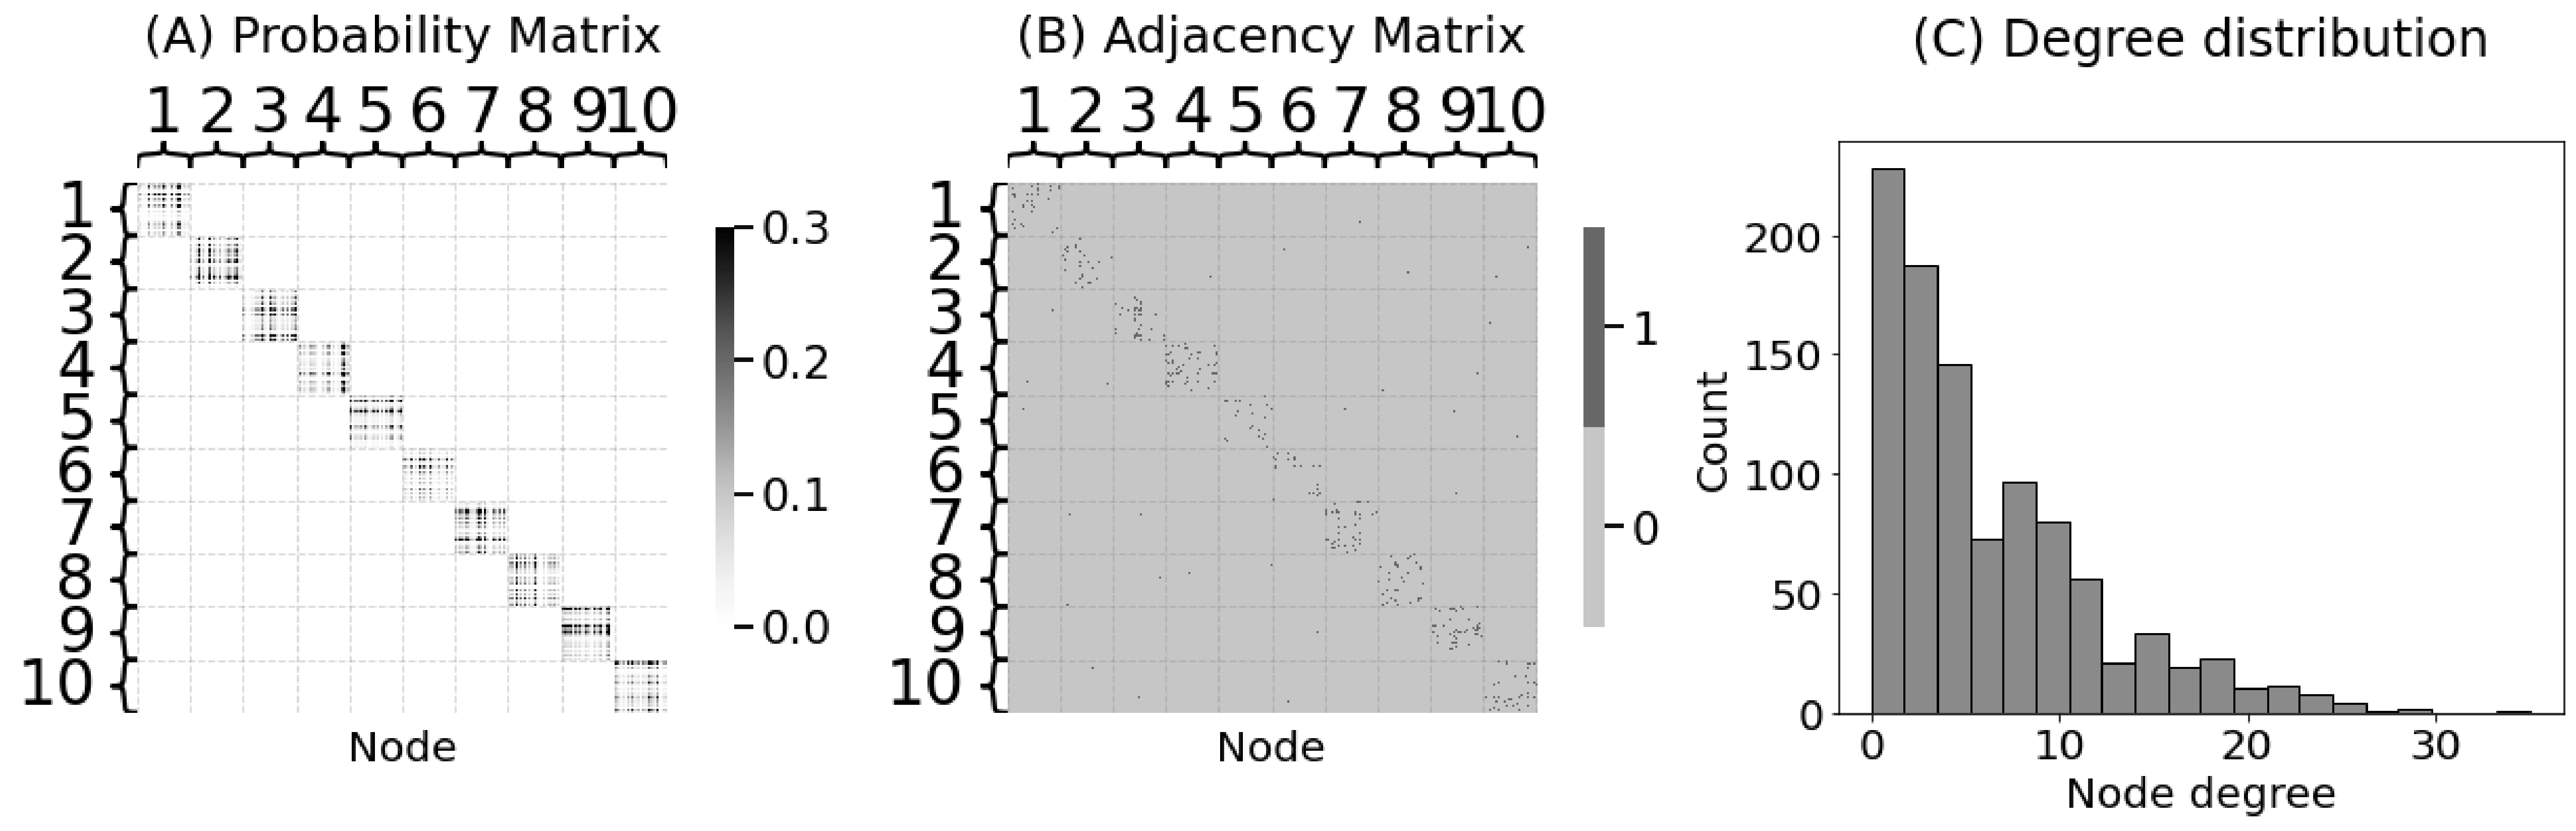
\includegraphics[width=\linewidth]{applications/ch7/Images/eigenspoke_ex.png}
    \caption[Network sample from sparse networks]{\textbf{(A)} the probability matrix, \textbf{(B)} the adjacency matrix, and \textbf{(C)} the heavy-tailed degree histogram for a network from a sparse sequence of networks.}
    \label{fig:ch7:density:deg}
\end{figure}

To do this, we're going to look at the top $5$ left singular vectors of the \texttt{DAD} Laplacian, remembering that \texttt{lse} is a function of these vectors (rescaled by the eigenvalues) in Algorithm \ref{alg:ch6:lse}. We will do this with \texttt{scipy}'s sparse \texttt{svd}, which we learned above is much faster for sparse data than a full \texttt{svd} with numpy:

\begin{lstlisting}[style=python]
import scipy as sp
from graspologic.utils import to_laplacian
from graspologic.plot import pairplot

# use sparse svd, so that we don't need to compute
# 1000 singular vectors and can just calculate the top 5
U, S, Vh = sp.sparse.linalg.svds(to_laplacian(A), k=5)
pairplot(U, labels=zs, title="Eigenspokes in the Laplacian")
\end{lstlisting}

We visualize the top $4$ singular vectors as a pairplot in Figure \ref{fig:ch7:density:pair}(A). Remember that each node is a point in this plot. What we notice is rather unusual. In many dimensions, such as dimensions $1$ and $2$ in particular, nodes appear to basically have an ``all or nothing'' pattern: entire communities of nodes have a $0$ for along almost all of the singular vectors, except for the long spoke that they stretch along. For instance, in dimension $2$, notice that the red community occupies the bottom of the dimension, and a combination of the pink, green, and blue communities occupy the top of the dimension. Likewise, along dimension $1$, we can see that the green community occupies the entire top of the dimension, and the yellow community occupies the entire bottom of the dimension. Along many of the other dimensions, such as $3$ and $4$, almost all of the nodes simply have a value of $0$. 

This ``all-or-nothing'' pattern is what is known as an \textit{EigenSpoke} \cite{Prakash2010}: some communities are clearly separated along axes, but have no separation along other axes. This all-or-nothing EigenSpoke behavior presents an extreme challenge for techniques like \texttt{KMeans} and \texttt{GMM}, which tend to favor spherical and elliptical ``blobs'' respectively.

\begin{figure}[h]
    \centering
    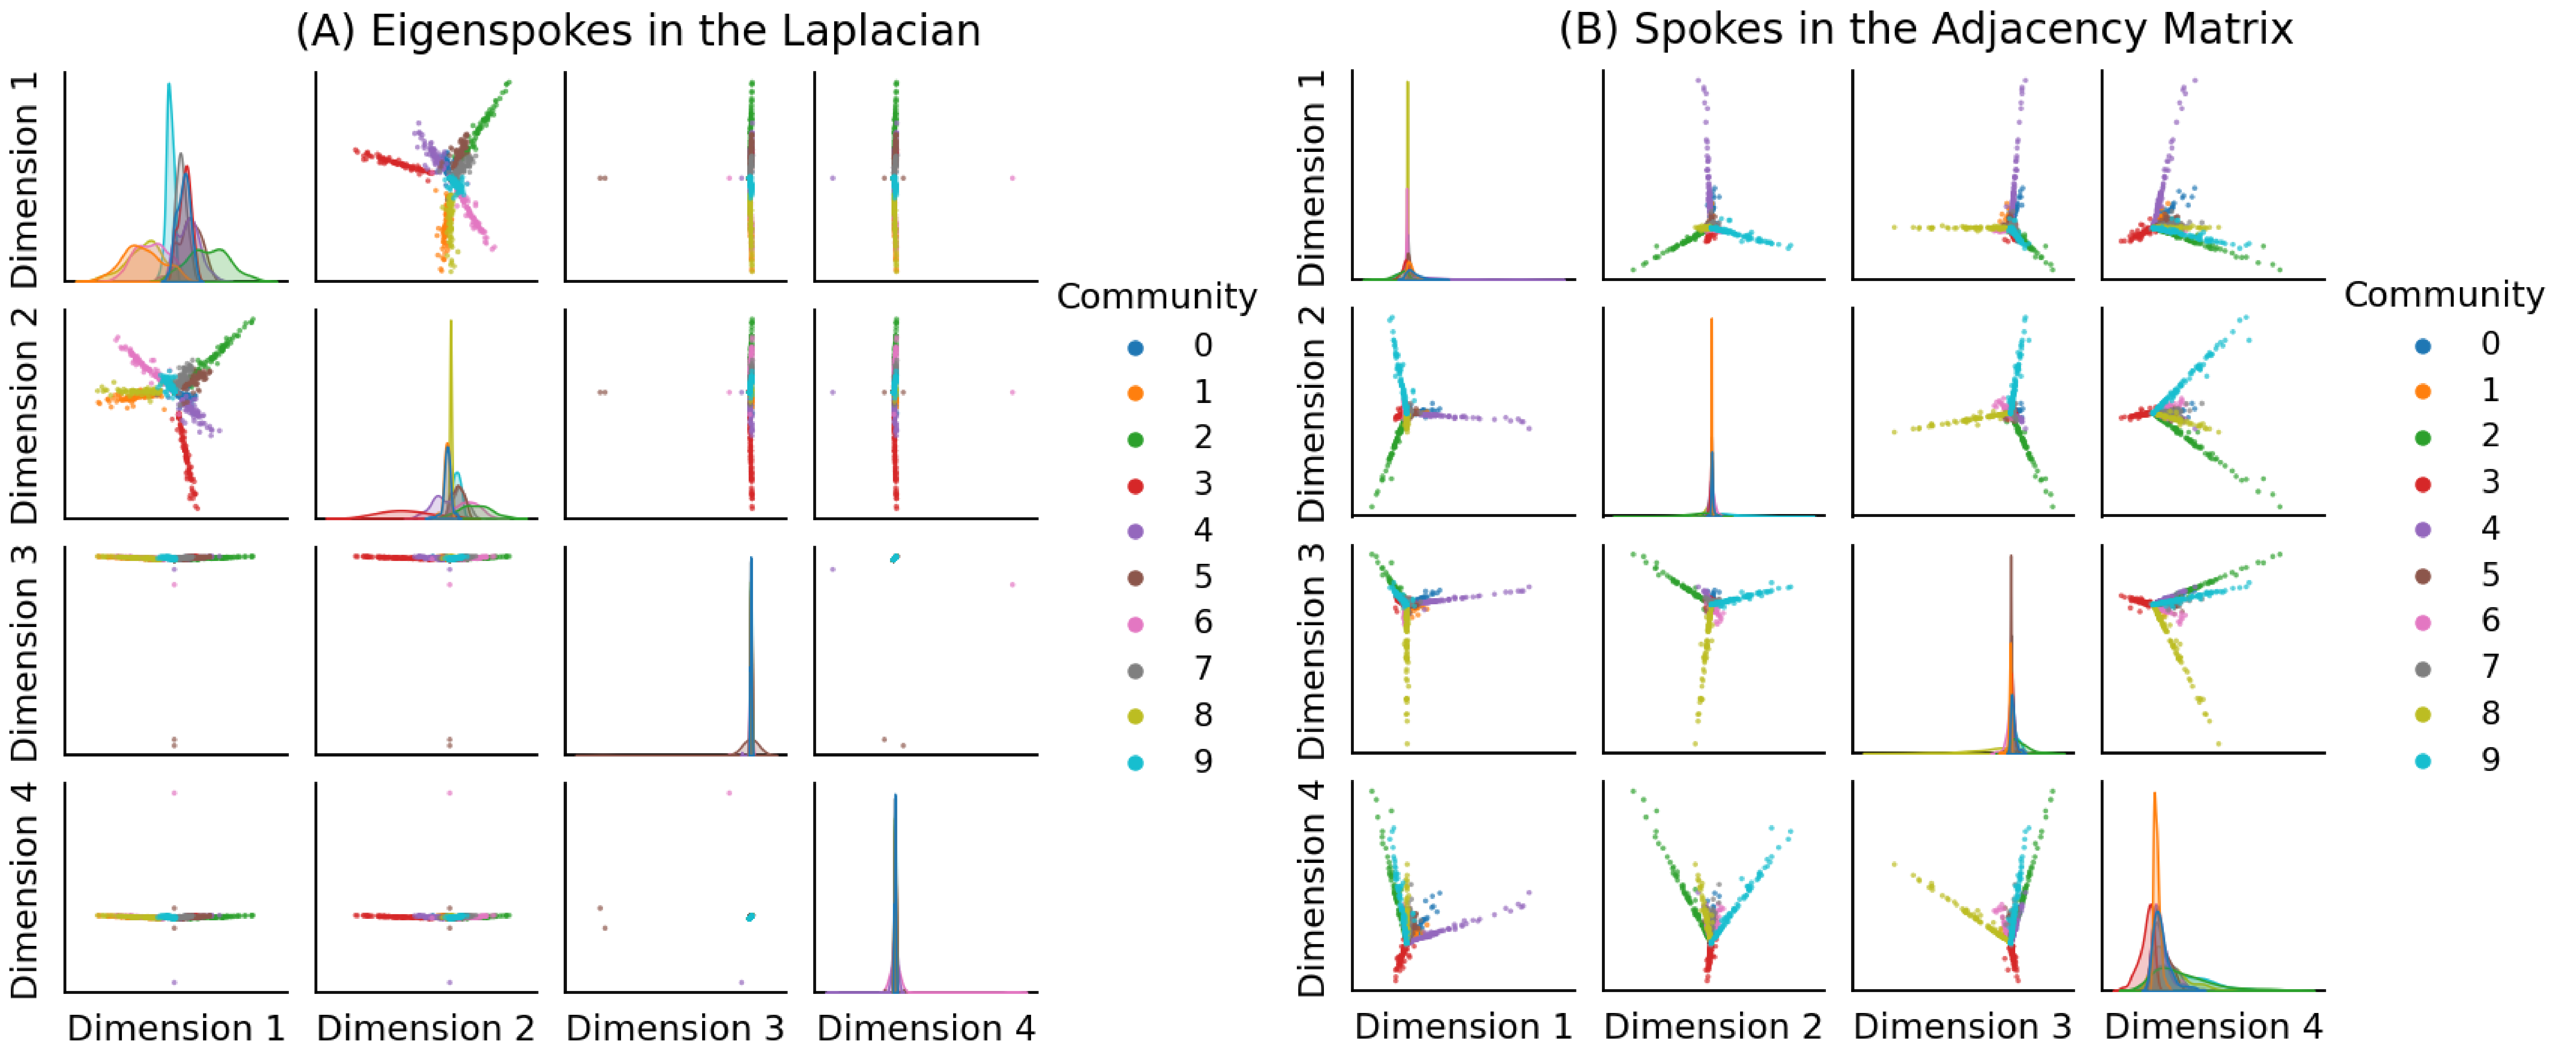
\includegraphics[width=\linewidth]{applications/ch7/Images/eigenspokes.png}
    \caption[Spokes in spectral embeddings of sparse adjacency matrices]{\textbf{(A)} Eigenspokes in the singular vectors of the laplacian, \textbf{(B)} moderate spokes in the singular vectors of the adjacency matrix.}
    \label{fig:ch7:density:pair}
\end{figure}

It seems pretty clear from the intuition that we gained in Section \ref{sec:ch7:comm_detect} that we don't appear to have the setup that \texttt{KMeans} or \texttt{GMM} do well in (structured blobs in the pairplots), so let's try looking at the singular vectors associated with the \texttt{ase} instead of the \texttt{lse}:

\begin{lstlisting}[style=python]
U, S, Vh = sp.sparse.linalg.svds(A, k=5)
pairplot(U, labels=zs, title="Eigenspokes in the Laplacian")
\end{lstlisting}

These aren't quite ``EigenSpokes'', in that the points aren't perfectly axis-aligned, but they're still quite spokey in shape. Here, too, naive community detection approaches will struggle, even though some of the communities look less poorly separated. To convince yourself as to why community detection with \texttt{kmeans} might fail, we would encourage you to visualize the distance matrix between pairs of nodes, like you did in Section \ref{sec:ch6:lse}, armed with the intuition that you gained in Section \ref{sec:ch7:comm_detect} about \texttt{kmeans} for community detection.

As it turns out, spectral approaches tend to struggle with networks that can be thought of as sparse (which, as we saw in Figure \ref{fig:ch7:density:sparsity}, it is). You can identify when you might run into these patterns by looking at how sparse the adjacency matrix is. You will typically run into sparse network troubles when the number of edges is ``on the order of'' the number of nodes in the network, and when it is far less than the number of potential edges in the network. You can calculate these with:

\begin{lstlisting}[style=python]
print("# Expected edges: {:2f}".format(np.triu(P).sum()))
print("# True edges: {:d}".format(np.triu(A).sum().astype(int)))
print("# Potential edges: {:d}".format(np.triu(np.ones((n, n))).sum().astype(int)))
# Expected edges: 3208.041454
# True edges: 3060
# Potential edges: 500500
\end{lstlisting}

When you run into situations where the number of edges is orders of magnitude less than the number of potential edges, you should be on the lookout for potentially running into sparsity concerns and be aware that many naive spectral techniques (such as \texttt{ase}, \texttt{lse}, and derived approaches like \texttt{mase} and \texttt{omni}) will struggle to produce embeddings that will facilitate downstream analysis (like community detection) \cite{Lei2013Dec}. You may need to turn to alternative techniques such as \cite{Krzakala2013Dec,Chen2012} to achieve high performance in these settings, where you incorporate different functions of the adjacency matrix that are better behaved for sparse regimes all together or apply penalties to nodes with low degrees to, in some sense, force your embeddings to avoid these spoke-like patterns.

\begin{floatingbox}[h]\caption{Simulating EigenSpokes is not an exact science}
EigenSpokes are a phenomena that arise in sparse networks, in that we have a good idea of what situations they can arise in (sparse networks) but not a great idea of how to reliably obtain them from random network samples. 

In this sense, you may have to run your simulations a few times to produce perfect ``EigenSpoke''-like patterns that run perfectly parallel along eigenvectors. They shouldn't be too hard to come by; when running these examples listed here, I tended to get spokes about $50\%$ of the time (and nonsensical embeddings in the other cases). 
\end{floatingbox}

\paragraph*{What does network sparsity have to do with these phenomena we observed with sparse adjacency matrices?}

The way that network sparsity fits into these strategies is a little bit indirect. First, we defined sparsity as a property that occurs over a sequence of random networks, which does not quite fit into real networks. Next, we showed that when a network had relatively few entries (its adjacency matrix was sparse), we could identify odd behaviors in particular algorithms, like the \texttt{lse} and \texttt{ase}. These two ideas feel at odds because the definition of sparsity does not apply to network samples, but in practice, we only have network samples.

Remember in Section \ref{sec:ch6:ase:whyuse}, we justified the \texttt{ase} by arguing that, when we have a network sample from a random network, as the network gets larger and larger, the estimated latent position matrix gets closer and closer to the true latent position matrix of the underlying random network. However, there is a caveat attached to this result: the underlying random network must have a probability matrix that obeys certain conditions \cite{Athreya2017Jan,Krzakala2013Dec} that ensure that the sequence of networks are not sparse. 

These conditions go a bit beyond the scope of this book, but the idea is that when the networks fail to satisfy these regimes, the naive \texttt{ase} loses its meaning. As the number of nodes increases, instead of the estimated latent position matrices getting closer and closer to the true latent position matrix of the underlying random network, the estimates become progressively more nonsensical. At some level, we lose the ability to say that $\hat X$ (the estimated latent position matrix) is a reasonable estimate of the true underlying latent position matrix $X$. This is why we observed ``puzzling'' behaviors in the spectral embeddings of our networks here (which were samples from a sparse sequence of random networks). 

\begin{floatingbox}[h]\caption{Complementary definitions of sparsity}
These two definitions of sparsity differ in that \textit{network sparsity} is a property of an underlying sequence of random networks, but \textit{matrix sparsity} is a property of the adjacency matrix (or a function thereof) for a network that you obtain. 

A network with a sufficiently sparse adjacency matrix will often run into problems associated with sparse sequences of random networks, and samples from sparse sequences of networks with enough nodes will often have sufficiently sparse adjacency matrices to cause odd results in network learning algorithms, so these two definitions prove complementary in network science.
\end{floatingbox}

\newpage